%% Template for the submission to:
%%   The Annals of Applied Statistics [AOAS]
%%
%%%%%%%%%%%%%%%%%%%%%%%%%%%%%%%%%%%%%%%%%%%%%%
%% In this template, the places where you   %%
%% need to fill in your information are     %%
%% indicated by '???'.                      %%
%%                                          %%
%% Please do not use \input{...} to include %%
%% other tex files. Submit your LaTeX       %%
%% manuscript as one .tex document.         %%
%%%%%%%%%%%%%%%%%%%%%%%%%%%%%%%%%%%%%%%%%%%%%%

\documentclass[aoas]{imsart}

%% Packages
\RequirePackage{amsthm,amsmath,amsfonts,amssymb}
\RequirePackage[authoryear]{natbib}
\usepackage{graphicx, hyperref, tikz, xcolor}
%\RequirePackage[colorlinks,citecolor=blue,urlcolor=blue]{hyperref}%% uncomment this for coloring bibliography citations and linked URLs
%\RequirePackage{graphicx}%% uncomment this for including figures

\startlocaldefs
%%%%%%%%%%%%%%%%%%%%%%%%%%%%%%%%%%%%%%%%%%%%%%
%%                                          %%
%% Uncomment next line to change            %%
%% the type of equation numbering           %%
%%                                          %%
%%%%%%%%%%%%%%%%%%%%%%%%%%%%%%%%%%%%%%%%%%%%%%
%\numberwithin{equation}{section}
%%%%%%%%%%%%%%%%%%%%%%%%%%%%%%%%%%%%%%%%%%%%%%
%%                                          %%
%% For Axiom, Claim, Corollary, Hypothesis, %%
%% Lemma, Theorem, Proposition              %%
%% use \theoremstyle{plain}                 %%
%%                                          %%
%%%%%%%%%%%%%%%%%%%%%%%%%%%%%%%%%%%%%%%%%%%%%%
%\theoremstyle{plain}
%\newtheorem{???}{???}
%\newtheorem*{???}{???}
%\newtheorem{???}{???}[???]
%\newtheorem{???}[???]{???}
%%%%%%%%%%%%%%%%%%%%%%%%%%%%%%%%%%%%%%%%%%%%%%
%%                                          %%
%% For Assumption, Definition, Example,     %%
%% Notation, Property, Remark, Fact         %%
%% use \theoremstyle{definition}            %%
%%                                          %%
%%%%%%%%%%%%%%%%%%%%%%%%%%%%%%%%%%%%%%%%%%%%%%
%\theoremstyle{definition}
%\newtheorem{???}{???}
%\newtheorem*{???}{???}
%\newtheorem{???}{???}[???]
%\newtheorem{???}[???]{???}
%%%%%%%%%%%%%%%%%%%%%%%%%%%%%%%%%%%%%%%%%%%%%%
%% Please put your definitions here:        %%
%%%%%%%%%%%%%%%%%%%%%%%%%%%%%%%%%%%%%%%%%%%%%%

\graphicspath{{../../output/figures/}}
\newcommand{\tablepath}{../../output/tables/}
\newcommand{\inputtable}[1]{\input{\tablepath #1}}
\newcommand{\defeq}{\stackrel{\text{def}}{=}}
\newcommand{\abs}[1]{\left\lvert#1\right\rvert}
\newcommand{\revision}[1]{{\color{orange} #1}}

\endlocaldefs

\begin{document}

\begin{frontmatter}
%%%%%%%%%%%%%%%%%%%%%%%%%%%%%%%%%%%%%%%%%%%%%%
%%                                          %%
%% Enter the title of your article here     %%
%%                                          %%
%%%%%%%%%%%%%%%%%%%%%%%%%%%%%%%%%%%%%%%%%%%%%%
\title{
  Sequential zero-sum games with mixed effects:\\
  An analysis of the pickoff limit in Major League Baseball
}
\runtitle{Analyzing the pickoff limit in Major League Baseball}

\begin{aug}
%%%%%%%%%%%%%%%%%%%%%%%%%%%%%%%%%%%%%%%%%%%%%%%
%% Only one address is permitted per author. %%
%% Only division, organization and e-mail is %%
%% included in the address.                  %%
%% Additional information such as            %%
%% identifying the corresponding author must %%
%% be included in in the Acknowledgments     %%
%% section if necessary.                     %%
%% ORCID can be inserted by command:         %%
%% \orcid{0000-0000-0000-0000}               %%
%%%%%%%%%%%%%%%%%%%%%%%%%%%%%%%%%%%%%%%%%%%%%%%
\author[A]{\fnms{Scott}~\snm{Powers}\ead[label=e1]{scott.powers@rice.edu}}
\author[B]{\fnms{Sivaramakrishnan}~\snm{Ramani}\ead[label=e2]{sivaramakrishnan.ramani@rice.edu}}
\author[A]{\fnms{Jacob}~\snm{Hahn}\ead[label=e3]{jacob.f.hahn@rice.edu}}
\author[B]{\fnms{Andrew J.}~\snm{Schaefer}\ead[label=e4]{andrew.schaefer@rice.edu}}
%%%%%%%%%%%%%%%%%%%%%%%%%%%%%%%%%%%%%%%%%%%%%%
%% Addresses                                %%
%%%%%%%%%%%%%%%%%%%%%%%%%%%%%%%%%%%%%%%%%%%%%%
\address[A]{Department of Sport Management, Rice University\printead[presep={,\ }]{e1,e3}}
\address[B]{Department of Computational Applied Mathematics and Operations Research, Rice University\printead[presep={,\ }]{e2,e4}}
\end{aug}

\begin{abstract}
  Recently, Major League Baseball (MLB) limited pitchers to three pickoff attempts, creating a cat-and-mouse game between pitcher and runner. Each failed attempt adds pressure on the pitcher to avoid using another, and the runner can intensify this pressure by extending their leadoff toward the next base. We model this dynamic as a two-player zero-sum sequential game in which the runner first chooses a lead distance, and then the pitcher chooses whether to attempt a pickoff. We establish optimality characterizations for the game and present variants of value iteration and policy iteration to solve the game. Using lead distance data, we estimate generalized linear mixed-effects models for pickoff and stolen base outcome probabilities given lead distance, context, and player skill. We compute the game-theoretic equilibria under the two-player model, as well as the optimal runner policy under a simplified one-player Markov decision process (MDP) model. In the one-player setting, our results establish an actionable rule of thumb: the Two-Foot Rule, which recommends that a runner increase their lead by two feet after each pickoff attempt.
\end{abstract}

\begin{keyword}
  \kwd{game theory}
  \kwd{hierarchical regression}
  \kwd{Markov decision process}
  \kwd{multilevel model}
  \kwd{sports analytics}
  \kwd{stochastic game}
\end{keyword}

\end{frontmatter}
%%%%%%%%%%%%%%%%%%%%%%%%%%%%%%%%%%%%%%%%%%%%%%
%% Please use \tableofcontents for articles %%
%% with 50 pages and more                   %%
%%%%%%%%%%%%%%%%%%%%%%%%%%%%%%%%%%%%%%%%%%%%%%
%\tableofcontents

%%%%%%%%%%%%%%%%%%%%%%%%%%%%%%%%%%%%%%%%%%%%%%
%%%% Main text entry area:


  
 \section{Introduction}
  \label{sec:introduction}
    On May 17, 2025, the Chicago Cubs hosted the Chicago White Sox in the second game of their Crosstown Series. In the bottom of the first inning, White Sox pitcher Sean Burke faced Cubs batter Michael Busch with two outs and Cubs runner Kyle Tucker on first base. Before the 1-1 pitch, Burke pivoted and threw to first base behind Tucker, who retreated safely before a tag. Tucker had 10 stolen bases in 10 attempts on the young season, the most of any base stealer who had not been caught \citep{fangraphs_major_2025}. On the White Sox broadcast, color commentator Steve Stone explained to the audience, ``The only problem is now there's two throws over there, and Tucker's gonna get a much bigger lead.'' On the next pitch, Tucker stole his 11$^\text{th}$ base of the season, the first Burke had allowed. ``I don't think anybody in the room could have thrown him out on that play,'' said Stone.

    For background, the stolen base is an exciting play in which a runner takes off on the pitch, attempting to reach the next base before the catcher can throw the ball to a fielder at the base to tag the runner out \citep{mlb_baseball_2025}. Whether attempting a stolen base or not, the runner takes a {\it lead} from their base, commonly positioning themselves 8--12 feet away from their base, toward the next base. The longer the lead, the shorter the distance needed to run to reach the next base. The pitcher's primary deterrent against long leads is a {\it pickoff attempt}, in which they throw the ball to a fielder at the runner's base, attempting a tag before the runner returns safely to the base.

    MLB stolen base totals surged in the 1980s and 1990s but then waned in the 2000s and 2010s as teams cut back on the play, which generally requires a high success rate in order to have a positive impact on run scoring \citep{tango_book_2007}. Before 2023, pickoff attempts could delay games because unsuccessful pickoff attempts do not advance the state of the game. Acknowledging this and other trends, MLB introduced several rule changes in 2023, with the goal of making the game more exciting \citep{castrovince_pitch_2023}. With these changes, a pitch clock limits the time between pitches, and there are restrictions on infielder positioning, curtailing defensive shifts. Two changes are particularly relevant to stolen base attempts: Bases are now wider (reducing the distance between first and second base by 4.5 inches), and there are now limitations on pickoff attempts, or more formally, {\it disengagements}.

    Under the new rules, pitchers are limited to three disengagements. When attempting a pickoff, instead of throwing a pitch, the pitcher disengages from the pitching rubber and throws the ball to the runner's base. If the pitcher disengages from the pitching rubber three times without successfully picking off the runner, then all runners automatically advance to the next base. Disengagements also include any time the pitcher steps off the rubber without attempting a pickoff, which we disregard in the present work. The disengagement count resets if a runner advances or if a plate appearance ends.

    This disengagement limit creates an interesting cat-and-mouse game between the pitcher and the runner. Each unsuccessful pickoff attempt disincentivizes the pitcher from attempting another pickoff, which incentivizes the runner to increase their lead distance. As indicated by Stone before the Tucker stolen base against the White Sox, players and coaches understand this intuitively. But how much should the runner extend their lead, and when should the pitcher attempt a pickoff? Our work introduces a formal model to address this timely question and the consequences arising from the implementation of our recommendations. % TODO: emphasize how this is an unresolved applied problem

    Figure \ref{fig:leads-overall} illustrates the difference in runner lead distance behavior (from first base) between 2022 and 2023. With zero disengagements in 2023, the distribution of lead distances is very similar to the overall distribution of lead distances in 2022. With each successive disengagement, we observe a positive shift in the distribution of lead distance in the 2023 data. In 2022, the average lead distance was 9.6 feet. In 2023, the average lead distance under zero, one, and two disengagements was 9.6 feet, 10.3 feet, and 11.0 feet, respectively.

    \begin{figure}
      \centering
      
\includegraphics[width = 0.8\textwidth]{leads_overall_light.pdf}
      \caption{
        \it The league-wide distribution of lead distance from first base when second base is unoccupied, comparing 2022 with 2023. The 2023 data are split by prior disengagements because, beginning in 2023, pitchers were limited to three disengagements, influencing pitcher and runner behavior. In 2022, there was no limit on the number of disengagements.
      }
      \label{fig:leads-overall}
    \end{figure}

    
    Section \ref{sec:sg-model} uses a two-player zero-sum sequential game to model the evolving interaction between the runner and the pitcher.  Our model captures the vital aspects of the play while retaining analytical and computational tractability. Our model is closely related to the class of stochastic/dynamic Stackelberg games \citep{goktas_zero-sum_2022,li_review_2017,lopez_stationary_2023,vasal_sequential_2022,vorobeychik_computing_2012}, which combines the elements of Stackelberg and stochastic games. The main difference between our infinite-horizon model and the stochastic Stackelberg games literature is that we do not discount the rewards. The rationale for this modeling choice is that our optimization objective---expected runs in the inning---by definition includes no discount. We establish a maximin Bellman equation for our sequential game and propose a variant of value iteration and policy iteration to determine the optimal strategies for runner and pitcher.

    In addition to developing a model which captures the important features of the pitcher-runner game, we analyze the model using recently available real-world MLB data. The most innovative component of our parameterization is the construction of transition probabilities. The outcome of each play is influenced by factors outside of our state variable, such as the sprint speed of the runner and the arm strength of the catcher. As a result, constructing transition probabilities using empirical conditional estimates (which use only the information from the current state and the actions of the player) is likely to be less accurate compared with a method that incorporates the player-specific factors.
    
    Section \ref{sec:transition-probability-model} uses a two-step procedure that includes the player-specific factors to estimate the transition probabilities. In the first step, we use a mixed-effects logistic regression model that calculates the probability of various runner outcomes taking into account the actions of the players and the player-specific information. Next, we construct an empirical probability distribution over the next state conditioned upon the current state, the runner outcomes, and the actions of the players. Finally, we determine the transition probability as the product of these two probabilities.

    Section \ref{sec:results} presents a numerical study on recent real-world data which illustrates that, relative to the optimal policy, observed pitcher and runner decisions are conservative. In current practice, pitchers attempt fewer pickoffs than optimal, and runners take shorter leads than optimal. Relative to observed behavior, optimal play would favor the offense slightly. Moreover, when restricting our model to a \revision{one}-player setup which allows agency only for the runner, the results reveal an actionable recommendation: the Two-Foot Rule, which recommends that a runner increase their lead by two feet after each pickoff attempt.

    \subsection{Related work}

    \citet{downey_pick_2015} analyzed pickoff throws and stolen base attempts as a mixed strategy game without using lead distance data. They modeled the two-player game as a simultaneous decision in which the pitcher chooses whether to attempt a pickoff and the runner chooses whether to attempt a stolen base, showing that this theoretical game has a mixed-strategy Nash equilibrium. Under this equilibrium, left-handed pitchers (typically possessing better pickoff moves than their right-handed counterparts) attempt fewer pickoffs and see fewer stolen bases attempted against them, a result validated by empirical data. In a later analysis, \citet{downey_pressure_2019} argued that pitchers can effectively implement a mixed strategy in low-pressure situations but struggle to randomize their decisions as pressure increases, showing a higher auto-correlation for sequential pickoff decisions in high-pressure situations. Both of these analyses covered a game in which pickoff attempts were unlimited.

    Several studies in the sports economics literature have examined the extent to which professional athletes play minimax strategy. \citet{palacios-huerta_professionals_2003} found evidence consistent with minimax equilibrium behavior in the mixed strategy game of the soccer penalty kick, in which the kicker chooses to shoot the ball left or right and the goalkeeper simultaneously chooses to dive left or right for the save. \citet{palacios-huerta_experientia_2008} followed this with a laboratory experiment featuring professional soccer players and college students simulating the penalty kick decision using cards, showing that the professionals played minimax but the students did not. On the other hand, \citet{kovash_professionals_2009} found evidence inconsistent with minimax equilibrium behavior in the National Football League (teams called more run plays and fewer pass plays than theoretically optimal) and in MLB (pitchers threw more fastballs than theoretically optimal).

    The history of quantitative analysis in baseball has deep roots in operations research (e.g., \citealp{lindsey_investigation_1963}; \citealp{freeze_analysis_1974}; \citealp{pankin_evaluating_1978}; \citealp{russell_devising_1994}; \citealp{bukiet_markov_1997}). The Markov process is particularly well suited for baseball, where the game's highly structured progression lends it well to an intuitive state space model \citep{sokol_intuitive_2004}. \citet{hirotsu_markov_2003} used a Markov model to inform substitution decision-making (specifically, pinch hitting) in baseball. The Markov process is also popular across sport analytics. \citet{hirotsu_using_2002} used a four-state Markov model for soccer to inform substitution decision-making based on how substitutions impact transition probabilities between states. Recently, \citet{chan_points_2021} used a Markov model to evaluate team performance in football. More specifically, the \revision{Markov decision process (MDP)} has become a particularly popular model in recent years for analyzing decision-making in sports, with applications in tennis \citep{nadimpalli_when_2013}, basketball \citep{sandholtz_markov_2020}, darts \citep{baird_optimising_2020} and football \citep{biro_reinforcement_2022}. In one particularly relevant baseball application, \citet{hirotsu_using_2019} used an MDP to model sacrifice bunt decisions on the basis of win probability, finding that the sacrifice bunt was more valuable than previously thought.

    An intermediate result of the present work is a probability model for stolen base attempts and successes (as well as an analysis of how those probabilities changed with the 2023 MLB rule changes), a topic which has not received much attention. \citet{loughin_assessing_2008} estimated linear mixed-effects models for stolen base attempts and successes, using random effects for pitcher and catcher (not the runner, notably) and fixed effects for balls, strikes, outs, score, venue and pitcher hand. They showed that the spread of pitcher effects is slightly greater than the spread of catcher effects. That analysis did not use data on runner sprint speed and catcher arm strength. More recently, \citet{stanley_modeling_2023} modeled stolen base success probability using both logistic regression and a random forest, including runner sprint speed and catcher arm strength as features but excluding player identities. That analysis was limited to data prior to the 2023 MLB rule changes that incentivized base stealing.
  
  \subsection{\revision{Data}}

    \revision{The new data which make it possible to address the lead distance problem are play-by-play lead distances measured via optical player tracking.} The runner's lead distance is defined as the distance between the runner's center of mass (projected onto the line between the first base and second base) and the nearest edge of first base. This distance is measured at the time of the pitcher's first movement\revision{, which could be a pitch or a pickoff attempt}. \revision{We obtained runner lead distances from MLB Advanced Media for every play in the 2022 and 2023 MLB regular seasons, covering the season before and the season after the rule change introducing the pickoff limit.} When the pitcher throws a pitch, the runner extends their lead by several feet from the time of the pitcher's first movement to the time of pitch release (known as taking a ``secondary lead''). \revision{However, the} data include only the lead distance at the time of the pitcher's first movement, not the secondary lead.

    \revision{In addition to the proprietary lead distance data, we} downloaded publicly available \revision{contextual data from the} MLB Stats API using the R package sabRmetrics \citep{powers_sabrmetrics_2025}. The dataset comprises 722,899 plays from the 2022 MLB regular season and 726,868 plays from the 2023 MLB regular season, where each play is either a pitch or a pickoff attempt (2.0\% pickoff attempts in 2022, 1.2\% in 2023). For each play, \revision{the data include bases occupied, ball-strike count, disengagements, and outs, as well as} identities of the pitcher, catcher, and runners involved. On each pickoff attempt, we observe whether it is successful. On each pitch, we observe whether the runner attempts a stolen base; and if so, we observe whether they are successful. On each pitch terminating a plate appearance, we observe the plate appearance outcome, such as strikeout, groundout, single, or home run.

    \revision{Finally, we obtained rich, publicly available data on catcher and runner skills measured via optical player tracking} \citep{baseball_savant_statcast_2024}. For each catcher-season, we observe {\it arm strength} (miles per hour), which Baseball Savant defines as the average of the top 10 percent (to capture peak performance) of throw speeds when the catcher is attempting to catch a base stealer. For each runner-season, we observe {\it sprint speed} (feet per second), which Baseball Savant defines as the average of the top 67 percent (to exclude low-effort plays) of peak running speeds on qualified runs: (1) home-to-first runs on weakly hit batted balls and (2) runs of two or more bases on balls hit into play (excluding runs from second base on extra-base hits).

  \subsection{\revision{Outline}}
  
    \revision{
      In Section \ref{sec:sg-model}, we present a theoretical model for the dynamic between runner and pitcher under the pickoff limit rule as a two-player sequential zero-sum game.
    }

  \section{Two-player sequential game model}
  \label{sec:sg-model}

    \revision{We begin with a theoretical model for a baseball inning that captures the vital aspects of the pitcher-runner game to} enable the generation of actionable insights for the runner and the pitcher. \revision{We take runs as the objective so that the runner aims to maximize expected runs scored until end of inning and the pitcher aims to minimize the same. Although game win probability would be a more pure objective, the choice of inning run expectation leads to more actionable insights, as we discuss in Section \ref{sec:discussion}.} Our model assumes a representative pitcher and a representative runner for the whole inning, rather than capturing full lineups and substitutions of players with varying skills. Without this assumption, we would end up with a nonstationary (infinite-horizon) two-player sequential game, which appears to be significantly more challenging to analyze when compared with the stationary version. The four components of our sequential game are as follows.

    {\it State space.} We use $s=(b,c,d,o) \in {\cal X}$ to capture a play, where     
    \begin{itemize}
      \item $b \in \{0, 1\}^3$ are the bases occupied by runners;
      \item $c \in \{0, 1, 2, 3\} \times \{0, 1, 2\}$ is the ball-strike count;
      \item $d \in \{0, 1, 2\}$ denotes the number of disengagements already used; and
      \item $o \in \{0, 1, 2\}$ denotes the number of outs.
    \end{itemize}
    The number of elements in ${\cal X}$ equals $2^3 \times (4 \times 3) \times 3 \times 3 = 864$. We use $\mathcal P$ to denote the set of four penultimate states and $\Delta$ to denote the terminal end-of-inning state. The purpose of the penultimate states is to keep track of the number of runs that are scored on the transition to the terminal state. A penultimate state $s \in \mathcal{P} \equiv \{0, 1, 2, 3\}$ represents the number of runs scored on the final play of the inning. We use $\mathcal{S} \equiv \mathcal{X} \cup \mathcal{P} \cup \{\Delta\}$ to denote the set of all states and $S_t$ to denote the state at play $t$ in a (fixed) inning. Traditionally, the state is defined by the bases occupied and the number of outs (24 non-terminal states) or by those and the ball-strike count (288 non-terminal states) \citep{bukiet_markov_1997}. Our construction of the state extends them by further including the number of disengagements as a component of the state, thereby allowing us to analyze the game under the new pickoff limit rule.

    {\it Action space.} We limit the agency of runners and pitchers to states in which only first base is occupied (i.e., the component $b$ in the state variable equals $(1,0,0)$). Although this restriction limits the scope, these states covered roughly $71\%$ of stolen base attempts in 2023. We emphasize that this  excludes the scenario with $b = (1, 0, 1)$ in which the first-base runner will often attempt a stolen base to lure a throw from the catcher, giving the third-base runner a chance to steal home and establishing a different dynamic \citep{miller_first-and-third_2024}. We leave this for future research.
    
    For states in which only first base is occupied, the first-base runner's action is the lead distance from first base, chosen in feet. The pitcher has only two actions: attempt a pickoff or throw a pitch. Formally, the action space of the first-base runner, $A_{\text{R}}$, and the action space of the pitcher, $A_{\text{P}}$, are as follows.
    
    \begin{align}
    \label{eqn:runner_action_space}
        A_\text{R}(s) \defeq \begin{cases}
            {\cal L} \text{ if } s = (b,c,d,o)\\
            \quad \text{ with } b = (1,0,0)\\
            \{\delta\} \text{ if } s = (b,c,d,o)\\
            \quad \text{ with } b \neq (1,0,0),\\
            \quad \text{ or } s \in {\cal P} \cup \{\Delta\}
        \end{cases} \forall s \in {\cal S},
    \end{align}
        
    where ${\cal L} \defeq [0,20]$ is the set of allowable lead distances for the first-base runner, and
    
    \begin{align}
      \label{eqn:pitcher_action_space}
      \begin{split}
        &A_{\text{P}}(s,a_\text{R}) \defeq
        \begin{cases}
          {\cal P} \text{ if } s = (b,c,d,o)\\
            \quad \text{ with } b = (1,0,0) \\
          \{\delta\} \text{ if } s = (b,c,d,o)\\
            \quad \text{ with } b \neq (1,0,0),\\
            \quad \text{ or } s \in {\cal P} {\cup} \{\Delta\},
        \end{cases}
        \forall s \in {\cal S}, a_\text{R} \in A_\text{R}(s),
      \end{split}
    \end{align} 
    where ${\cal P} \defeq \{0,1\}$, with $p = 1$ corresponding to a pickoff attempt and $0$ otherwise.  Here, $\delta$ is a dummy element that captures the lack of agency. We note that the state of our sequential game progresses even when no actions are played by both players. We will model this through appropriate transition probabilities.  

    {\it Transition probabilities.} The uncertainty in our sequential game is modeled through transition probabilities, i.e., the conditional probability of transitioning to a future state given the sequence of previously visited states and the actions played in those states. Our sequential game assumes that the transition probabilities satisfy the Markov property.  Following the convention in the literature, we denote the transition probability as $p(\cdot \mid s,a_\text{R},a_\text{P}) \ \forall s \in {\cal S}, a_\text{R} \in A_\text{R}(s), a_\text{P} \in A_\text{P}(s,a_\text{R})$. Section \ref{sec:transition-probability-model} details our specific construction of transition probabilities, which uses generalized linear mixed-effects models to estimate runner outcome (e.g., unsuccessful pickoff attempt or successful stolen base attempt) probabilities which depend on lead distance and the pitcher's pickoff decision, as well as player-specific factors. These, along with appropriate conditional empirical frequencies, will be used to construct the transition probabilities.

    {\it Reward function.} The final component of our sequential game is the reward function, which models the payoff received by the players. Since we use a  zero-sum sequential game, the payoff obtained by one player comes at the expense of the other player. We choose the number of runs scored as the reward function. This design choice is more suitable for the early and middle innings of a game and less suitable for the later innings, particularly the bottom of the ninth or extra innings, when the offense knows how many runs they need to score to win the game. For any state $s \in {\cal S}$, the reward function captures the number of runs scored by the batting team in transitioning from state $s$ to $s'$ given the actions of the first-base runner and the pitcher. Formally,
    \begin{align}
      \label{eqn:runner_pitcher_reward}
        r(s'|s,a_\text{R},a_\text{P}) &\defeq r(s'|s) \\
        \nonumber
        \quad 
        \forall s,s' \in {\cal S},\, a_\text{R} \in A_\text{R}(s),\, & a_\text{P} \in A_\text{P}(s,a_\text{R}),
    \end{align}
    where
    \begin{align}
      \label{eqn:common_reward}
      r(s'|s) \defeq  \begin{cases}
          (g(b) + o) - (g(b') + o') +\\ \quad \mathbb{I}\{c' = (0, 0),\, d' = 0\} \text{ if } s,\, s' \in \mathcal{X}\\
          s'  \text{ if } s \in \mathcal{X},\, s' \in \mathcal{P}\\
          0  \text{ if } s' = \Delta,
      \end{cases} 
    \end{align}
    where $g: \{0, 1\}^3 \rightarrow \{0, 1, 2, 3\}$ counts the number of runners on base. Note that our reward function in \eqref{eqn:runner_pitcher_reward} depends only on the current state and the next state, and not on the actions of the first-base runner or the pitcher. The formula in \eqref{eqn:common_reward} infers the number of runs scored by counting the offensive players captured by the states before and after the transition. If the transition corresponds to the end of a plate appearance (i.e. $c' = (0, 0),\, d' = 0$), then we account for one more offensive player (the batter) in the next state. Since the number of runs scored on the last play cannot be uniquely determined from the current state, we use the penultimate states to track the number of runs scored on the last play. We note that our transition probabilities will be constructed such that these penultimate states transition to the terminal end-of-inning state with probability $1$. Since the reward function \eqref{eqn:runner_pitcher_reward} depends only on the current and the next state, it appears to be independent of the actions of the players. However, the next state to which our sequential game transitions is (probabilistically) determined by the actions of both the players through the transition probabilities, thereby making the rewards depend indirectly on the actions of both players.

    Our sequential game models the progression of an inning as follows. Let $s \in {\cal S}$ denote the state of the sequential game from which a play begins. Upon observing this state, the first-base runner picks an action $a_\text{R} \in A_\text{R}(s)$. The pitcher observes the state $s$ and the first-base runner's action $a_\text{R}$, and then picks an action $a_\text{P} \in A_\text{P}(s,a_\text{R})$. After playing $a_\text{R}$ and $a_\text{P}$, the sequential game then transitions into state $s'$ with probability $p(s'|s,a_\text{R},a_\text{P})$ and the batting team collects a reward $r(s'|s,a_\text{R},a_\text{P})$ in the zero-sum game. A play then begins from $s'$, and the process repeats. The goal of the batting team is to maximize (through the actions of the first-base runner) the expected total rewards over the plays in the inning while the goal of the fielding team is to minimize (through the actions of the pitcher) the expected total rewards obtained by the batting team.

    Intuitively, any sound strategy for the first-base runner and the pitcher depends on the state of the sequential game (for the pitcher, it also depends on the actions played by the first-base runner). This is formally captured using the concept of policy. A (deterministic, stationary) policy for the first-base runner is a decision-rule that prescribes the action to be played in every possible state. Similarly, a (deterministic, stationary) policy for the pitcher is a decision-rule that prescribes the action to be played for every possible state and the corresponding actions of the first-base runner in those states. A mathematical treatment of policies is presented in the Appendix. We denote the set of policies for the runner and pitcher by $\Pi_\text{R}$ and $\Pi_\text{P}$, respectively.

    The concept of policies allows us to mathematically characterize the runs scored in an inning. Suppose the first-base runner and the pitcher employ policies $\pi_\text{R} \in \Pi_\text{R}$ and $\pi_\text{P} \in \Pi_\text{P}$, respectively. Assuming the play starts from a state $s \in {\cal S}$, the expected total runs scored (by the batting team) in an inning then equals 
    \begin{align}
       \label{eqn:sg_pol_val}
       V^{\pi_\text{R},\pi_\text{P}}(s) &\defeq \mathbb{E}^{\pi_\text{R},\pi_\text{P}}\Bigg[\sum_{t=0}^\infty r(S_{t+1}|S_t) \Big| S_0 = s\Bigg], 
       % \nonumber
       % &\quad \forall s \in {\cal S},
    \end{align}
    % TODO: Fix missing lemma number
    where $\mathbb{E}^{\pi_\text{R},\pi_\text{P}}$ denotes the expectation with respect to the distribution induced by $\pi_\text{R}$ and $\pi_{\text{P}}$. Observe that, unlike the typical sequential games studied in the literature, we do not discount the rewards. This is because our optimization objective is rest-of-inning expected runs, which by definition does not discount runs scored on later plays. Though the undiscounted case is more realistic in our setup, it might lead to technical issues since $V^{\pi_\text{R},\pi_\text{P}}(s)$ in \eqref{eqn:sg_pol_val} can potentially be infinite. However, all innings eventually end. As a result, the infinite series appearing inside the expectation in the right-hand side of \eqref{eqn:sg_pol_val} can be approximated with arbitrary precision by truncating the sum at some finite $T \in \mathbb{N}$, and hence we can expect $V^{\pi_\text{R},\pi_\text{P}}(s)$ to take finite values. This reasoning is rigorously justified in Lemma \ref{lem:sg_pol_val_well_defined} in the Appendix. Therefore, in the rest of the paper, we take $V^{\pi_\text{R},\pi_\text{P}}(s)$ to be a finite number for all $\pi_\text{R} \in \Pi_\text{R}, \pi_\text{P} \in \Pi_\text{P}$, and $s \in {\cal S}$. 
   
    The goal of the batting team is to select a policy that will maximize the expected total runs scored by them. At the same time, the fielding team minimizes the expected total runs scored by the batting team by employing a suitable policy. Taking the rational behavior of both the players into account, the maximum runs scored by the batting team when a play begins from state $s \in {\cal S}$ is given as 
    \begin{equation}
    \label{eqn:sg_val}
      V^*(s) \defeq \max_{\pi_\text{R} \in \Pi_\text{R}}\min_{\pi_\text{P} \in \Pi_\text{P}}V^{\pi_\text{R},\pi_\text{P}}(s) \ \forall s \in S.
    \end{equation}
    We call $V^*$ the \emph{optimal value function}. In our context, $V^*$ is the maximum expected total runs scored in an inning by the batting team, which, by the zero-sum property of the game, equals the minimum expected total runs incurred by the fielding team. A policy pair $(\pi_\text{R}^*,\pi_\text{P}^*) \in \Pi_\text{R} \times \Pi_\text{P}$ such that $V^{\pi_\text{R}^*,\pi_\text{P}^*}(s) = V^*(s) \ \forall s \in {\cal S}$ is called an equilibrium policy. That is, $\pi_\text{R}^*$ is a policy for the batting team that maximizes the expected total runs scored by them, and $\pi_\text{P}^*$ is a policy for the fielding team that minimizes the expected total runs incurred by them. In other words, $\pi_\text{R}^*$ is an optimal policy for the batting team and $\pi_\text{P}^*$ is an optimal policy for the fielding team. 

    A characterization of optimality conditions for \eqref{eqn:sg_val} including a dynamic programming equation is presented in the Appendix. In our computational experiments in Section \ref{sec:results}, we use value iteration to solve \eqref{eqn:sg_val}. The value iteration algorithm is as follows. Starting from an arbitrary $V^0 \in \mathbb{R}^{\abs{\cal S}}$ with $V^0(\Delta) = 0$, iteratively obtain $V^k$ via the following updates
    \begin{align}
    \label{eqn:vi_algorithm}
      V^k(s) &\defeq \max_{a_\text{R} \in A_\text{R}(s)} \min_{a_\text{p} \in A_\text{P}(s,a_\text{R})}\sum_{s' \in \mathcal{S}}[r(s'|s) + V^{k-1}(s')] p(s'|s,a_\text{R},a_\text{P}) \quad \forall s \in \mathcal{S}.
    \end{align}
    % TODO: Decide what is meant by an informal theorem and format this accordingly.
    {\bf Theorem 1} (Informal) {\it 
    The iterates $V^k$ generated in \eqref{eqn:vi_algorithm} converge to the optimal value function $V^*$.}
     
    \noindent This result is proved in the Appendix. Furthermore, the proof of Theorem 1 also establishes a convergence rate of the form $\abs{V^k(s) - V^*(s)} \leq O(\rho^k)$ for all $s \in {\cal S}$ and a $\rho \in (0,1)$.
    
    We note that fixing a pitcher policy reduces our two-player sequential game to a \revision{one}-player MDP whose objective is to optimize the lead distance for the first-base runner. Optimality criterion similar to the two-player sequential game also exists for MDP with undiscounted rewards \citep[Section 7.2]{bertsekas_dynamic_2012}. Numerical experiments using this decision  model for a specific pitcher policy are presented in Section \ref{sec:results-one-player}. These results may provide more immediately actionable insights for lead distance selection, as we discuss in Section \ref{sec:discussion}.

  \section{\revision{Hierarchical} transition probability model}
  \label{sec:transition-probability-model}

    \revision{
      To infer the two-player sequential game model using empirical data, it is critical to estimate the transition probabilities $p(\cdot \mid s,a_\text{R},a_\text{P})$. In other words, we must understand how the runner's chosen lead distance and the pitcher's chosen action (pickoff or pitch) influence the stochastic transitions between game states. For states with trivial action space ($a_\text{R} = a_\text{P} = \delta$), we simply use the empirical transition probabilities between states observed in the data. For more intersting states, we decompose the state transition into (1) a runner outcome and (2) a conditional state transition, given the runner outcome. While the runner outcome depends on runner and pitcher actions, we assume that the state transition is conditionally indepedent of the actions, given the runner outcome. In other words, the actions only influence the state transition through the runner outcome. We address the validity of this assumption in Section \ref{sec:sensitivity}.
      % TODO: Add a section addressing validity of assumptions
    }

    Throughout \revision{this section}, we use $s_i = (b_i, c_i, d_i, o_i)$ to denote the state of the game at the beginning of each observed play $i \in \{1, ..., n\}$ (which can be a pitch or a pickoff attempt). We use $\mathcal{H}^R$, $\mathcal{H}^P$, and $\mathcal{H}^C$ to denote the sets of runners, pitchers and catchers, respectively. On play $i$:
    \begin{itemize}
      \item $h_i^R \in \mathcal{H}^R$ is the runner;
      \item $h_i^P \in \mathcal{H}^P$ is the pitcher;
      \item $h_i^C \in \mathcal{H}^C$ is the catcher;
      \item $z_i^R \in \mathbb{R^+}$ is the sprint speed of runner $h_i^R$; and
      \item $z_i^C \in \mathbb{R^+}$ is the arm strength of catcher $h_i^C$.
    \end{itemize}
    
    When the play begins, we use $\ell_i \in \mathbb{R}^+$ to denote the lead distance (in feet) taken by the first-base runner; and we use $p_i \in \{0, 1\}$ to denote whether the pitcher attempts (1) or does not attempt (0) a pickoff. We use $r_i \in \{\mbox{P}^+,\, \mbox{P}^-,\, \mbox{S}^+,\, \mbox{S}^-,\, \mbox{N}\} \equiv \mathcal{R}$ to denote the runner outcome, where
    \begin{itemize}
      \item $\mbox{P}^+$ represents a successful pickoff attempt (runner is out);
      \item $\mbox{P}^-$ represents an unsuccessful pickoff attempt (runner is safe);
      \item $\mbox{S}^+$ represents a successful stolen base attempt (runner is safe);
      \item $\mbox{S}^-$ represents an unsuccessful stolen base attempt (runner is out); and
      \item $\mbox{N}$ represents no runner action (a pitch with no stolen base attempt).
    \end{itemize}
    If there is no runner on first base, then $\ell_i$ and $r_i$ are undefined.
    
    \revision{
      Using $\mathcal{E}$ to denote the event $\{S_i = s, \ell_i = a_\text{R}, p_i = a_\text{P}\}$ for states $s$ with nontrivial action space, the law of total probability decomposes the transition probability function as
      \begin{align}
        \label{eqn:prob-state-transition-two-player}
          p(s'|s,\, a_\text{R},\, a_\text{P}) = \mathbb{P}(S_{i+1} = s' \mid \mathcal{E}) = \sum_{r \in \mathcal{R}} \big(\mathbb{P}(R_i = r \mid \mathcal{E}) \cdot \mathbb{P}(S_{i+1} = s' \mid \mathcal{E},\, R_i = r)\big).
      \end{align}
      In Section \ref{sec:prob-runner-outcome}, we explain the inference of the runner outcome probability $\big(\mathbb{P}(R_i = r \mid \mathcal{E})$, and in Section \ref{sec:prob-state-transition}, we explain the inference of the conditional state transition probability $\mathbb{P}(S_{i+1} = s' \mid \mathcal{E},\, R_i = r)$.
    }

    \subsection{\revision{Runner outcome model}}
    \label{sec:prob-runner-outcome}

      There are $|\mathcal{R}| = 5$ possible outcomes for the runner with respect to the run game, \revision{and they have a hierarchical structure illustrated by Figure \ref{fig:runner-outcome-tree}. We leverage this hierarchy to decompose the runner outcome probability into four components.} Using $R_i$ to denote the random variable governing the probability distribution over $r_i$,
      \begin{itemize}
        \item $\phi_i = \mathbb{P}(R_i \in \{\mbox{P}^+,\, \mbox{P}^-\})$ is the pickoff attempt probability;
        \item $\phi_i^+ = \mathbb{P}(R_i \in \{\mbox{P}^+\} \mid R_i \in \{\mbox{P}^+,\, \mbox{P}^-\})$ is the pickoff success probability;
        \item $\psi_i = \mathbb{P}(R_i \in \{\mbox{S}^+,\, \mbox{S}^-\} \mid R_i \in \{\mbox{S}^+,\, \mbox{S}^-, N\})$ is the stolen base attempt probability; and
        \item $\psi_i^+ = \mathbb{P}(R_i \in \{\mbox{S}^+\} \mid R_i \in \{\mbox{S}^+,\, \mbox{S}^-\})$ is the stolen base success probability.
      \end{itemize}

      \revision{
        \begin{figure}
          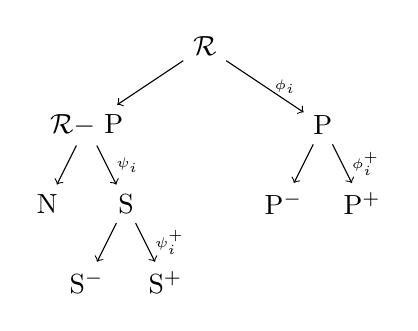
\begin{tikzpicture}
            \node (R)  at ( 0.0,  0) {$\mathcal{R}$};
            \node (P)  at ( 1.5, -1) {P};
            \node (RP) at (-1.5, -1) {$\mathcal{R} -$ P};
            \node (P+) at ( 2.0, -2) {P$^+$};
            \node (P-) at ( 1.0, -2) {P$^-$};
            \node (S)  at (-1.0, -2) {S};
            \node (N)  at (-2.0, -2) {N};
            \node (S+) at (-0.5, -3) {S$^+$};
            \node (S-) at (-1.5, -3) {S$^-$};
            \draw[->] (R)  -- node[right] {\tiny $\phi_i$} (P);
            \draw[->] (R)  -- (RP);
            \draw[->] (P)  -- node[right] {\tiny $\phi_i^+$} (P+);
            \draw[->] (P)  -- (P-);
            \draw[->] (RP) -- node[right] {\tiny $\psi_i$} (S);
            \draw[->] (RP) -- (N);
            \draw[->] (S)  -- node[right] {\tiny $\psi_i^+$} (S+);
            \draw[->] (S)  -- (S-);
          \end{tikzpicture}
          \caption{
            \revision{
              \it A diagram of the runner outcome hierarchy. P represents \{P$^+$, P$^-$\}, and S represents \{S$^+$, S$^-$\}. Each right-moving edge is labeled with the conditional probability of the right child node given the parent node. The conditional probability of the left child is one minus the conditional probability of the right child.
            }
          }
          \label{fig:runner-outcome-tree}
        \end{figure}

        Each of these probabilities depends on the play's contextual covariates and player skills, for which the subscript $i$ accounts. If the pitcher has agency, then the pickoff attempt probability depends only on pitcher action, $\phi_i = p_i$. However, it is useful for some applications to remove the pitcher's agency, as described in Section \ref{sec:prob-po-attempt}, so we keep the notation general. The runner outcome probability comprises the products of the component probabilities:
        \begin{align}
          \label{eqn:prob-runner-outcome-two-player}
          \begin{split}
            \mathbb{P}(R_i = r \mid \mathcal{E}) =
            \begin{cases}
              \phi_i \cdot \phi_i^+                            & \mbox{if } r = \mbox{P}^+\\
              \phi_i \cdot (1 - \phi_i^+)                      & \mbox{if } r = \mbox{P}^-\\
              (1 - \phi_i) \cdot \psi_i \cdot \psi_i^+         & \mbox{if } r = \mbox{S}^+\\
              (1 - \phi_i) \cdot \psi_i \cdot (1 - \psi_i^+)   & \mbox{if } r = \mbox{S}^-\\
              (1 - \phi_i) \cdot (1 - \psi_i)                  & \mbox{if } r = \mbox{N}\\
            \end{cases}.
          \end{split}
        \end{align}
      }

      \revision{We estimate the component binomial outcome probabilities using} generalized linear mixed-effects models (GLMMs, \citealp{stroup_generalized_2012}). Mixed-effects models allow us to incorporate player random effects along with fixed effects for game state variables and lead distance. Player random effects are particularly appropriate for this setting because they yield player skill estimates which go beyond measurable characteristics like sprint speed and are regularized towards a common mean. \revision{Sections \ref{sec:prob-po-attempt} through \ref{sec:prob-sb-success} detail the model specifications.}

      \subsubsection{Pickoff attempt probability}
      \label{sec:prob-po-attempt}

        \revision{
          In the two-player sequential game model, there is no need to estimate pickoff attempt probability because it is a deterministic decision made by the pitcher. However, as we discuss in Section \ref{sec:discussion}, modeling the pickoff decision as stochastic rather than antagonistic results in different, and perhaps more immediately actionable, insights for the runner. From the runner's perspective, this approach models the pitcher's action as a stochastic response to the runner's lead distance. In this section we present a probability model for pickoff attempts, which forms the basis for the results in Section \ref{sec:results-one-player}.
        }

        We model $\phi_i$ using a mixed-effects logistic regression with fixed effects for balls, strikes, outs, disengagements (as a categorical), and lead distance; and with a random effect for the pitcher.
        \begin{align}
          \label{eqn:prob-po-attempt}
          \begin{split}
            \log\left(\frac{\phi_i}{1 - \phi_i}\right) &= \alpha + \beta^B c_i^B + \beta^S c_i^S +
              \beta^O o_i + \beta^D_{d_i} + \beta^L \ell_i + \gamma^P_{h_i^P}\\
            \gamma^P_{h} &\sim \mathcal{N}(0, \sigma^2_P) \hspace{4mm} \mbox{\it i.i.d.} \hspace{4mm} \forall h \in \mathcal{H}^P.
          \end{split}
        \end{align}
        This model has seven fixed, unknown parameters: the intercept $\alpha$; the five slopes $\beta^B$, $\beta^S$, $\beta^O$, $\beta^D$, and $\beta^L$; and the variance parameter $\sigma^2_P$. The number of random effects is $|\mathcal{H}^P|$\revision{, and we interpret them as latent individual tendencies to attempt pickoffs.}
        
      \subsubsection{Pickoff success probability}
      \label{sec:prob-po-success}

        We model $\phi_i^+$ using a mixed-effects logistic regression with a fixed effect for lead distance and a random effect for pitcher.
        \begin{align}
          \label{eqn:prob-po-success}
          \begin{split}
            \log\left(\frac{\phi_i^+}{1 - \phi_i^+}\right) &= \alpha + \beta^L \ell_i + \gamma^P_{h_i^P},\\
            \gamma^P_{h} &\sim \mathcal{N}(0, \sigma^2_P) \hspace{4mm} \mbox{\it i.i.d.} \hspace{4mm} \forall h \in \mathcal{H}^P.
          \end{split}
        \end{align}
        This model has three fixed, unknown parameters: the intercept $\alpha$, the slope $\beta^L$, and the variance parameters $\sigma^2_P$. The number of random effects is $|\mathcal{H}^P|$\revision{, and we interpret them as latent individual pickoff skill.}

      \subsubsection{Stolen base attempt probability}
      \label{sec:prob-sb-attempt}

        Modeling the runner's decision to attempt a stolen base \revision{presents empirical challenges. While classical game theory might frame this as a deterministic decision, this model aligns poorly with real-life decisions made by baserunners. We posit that the decision is a response to latent environment variables (e.g., the pitcher's body language or timing between pitches) that we do not observe in the data available. Therefore, we treat the decision as stochastic given player skills and contextual factors. Further, we exclude lead distance from this model to avoid a paradoxical situation in which the optimal action for the runner would be to shorten their lead to reduce the probability of an ill-advised stolen base attempt.}

        We model $\psi_i$ using a mixed-effects logistic regression with fixed effects for balls, strikes, outs, disengagements (as a categorical), runner sprint speed, and catcher arm strength; and with random effects for runner, pitcher, and catcher.
        \begin{align}
          \label{eqn:prob-sb-attempt}
          \begin{split}
            \log\left(\frac{\psi_i}{1 - \psi_i}\right) &= \alpha + \beta^B c_i^B + \beta^S c_i^S +
              \beta^O o_i + \beta^D_{d_i} + (\beta^R z_i^R + \gamma^R_{h_i^R}) +
              \gamma^P_{h_i^P} + (\beta^C z_i^C + \gamma^C_{h_i^C}),\\
            \gamma^R_{h} &\sim \mathcal{N}(0, \sigma^2_R) \hspace{4mm} \mbox{\it i.i.d.} \hspace{4mm} \forall h \in \mathcal{H}^R,\\
            \gamma^P_{h} &\sim \mathcal{N}(0, \sigma^2_P) \hspace{4mm} \mbox{\it i.i.d.} \hspace{4mm} \forall h \in \mathcal{H}^P,\\
            \gamma^C_{h} &\sim \mathcal{N}(0, \sigma^2_C) \hspace{4mm} \mbox{\it i.i.d.} \hspace{4mm} \forall h \in \mathcal{H}^C.
          \end{split}
        \end{align}
 
        We interpret $(\beta^R z_i^R + \gamma^R_{h_i^R})$ as the effect of runner $h_i^R$ on the attempt probability, combining the effect of the runner's \revision{measured} sprint speed with \revision{a latent effect representing the individual's tendency to attempt a steal}. By including a fixed effect for sprint speed, we are effectively regularizing the runner effects toward priors based on their sprint speeds. The interpretation of $(\beta^C z_i^C + \gamma^C_{h_i^C})$ for catchers is similar: Each catcher has an estimated effect regularized toward a prior based on their arm strength.
      
      \subsubsection{Stolen base success probability}
      \label{sec:prob-sb-success}

        We model $\psi_i^+$ using a mixed-effects logistic regression with fixed effects for lead distance, runner sprint speed, and catcher arm strength; and with random effects for runner, pitcher, and catcher.
        \begin{align}
          \label{eqn:prob-sb-success}
          \begin{split}
            \log\left(\frac{\psi_i^+}{1 - \psi_i^+}\right) &= \alpha + \beta^L \ell_i + (\beta^R z_i^R + \gamma^R_{h_i^R}) +
              \gamma^P_{h_i^P} + (\beta^C z_i^C + \gamma^C_{h_i^C}),\\
            \gamma^R_{h} &\sim \mathcal{N}(0, \sigma^2_R) \hspace{4mm} \mbox{\it i.i.d.} \hspace{4mm} \forall h \in \mathcal{H}^R,\\
            \gamma^P_{h} &\sim \mathcal{N}(0, \sigma^2_P) \hspace{4mm} \mbox{\it i.i.d.} \hspace{4mm} \forall h \in \mathcal{H}^P,\\
            \gamma^C_{h} &\sim \mathcal{N}(0, \sigma^2_C) \hspace{4mm} \mbox{\it i.i.d.} \hspace{4mm} \forall h \in \mathcal{H}^C.
          \end{split}
        \end{align}
        As in (\ref{eqn:prob-sb-attempt}), we interpret $(\beta^R z_i^R + \gamma^R_{h_i^R})$ as the runner effect regularized toward a prior based on sprint speed and $(\beta^C z_i^C + \gamma^C_{h_i^C})$ as the catcher effect regularized toward a prior based on arm strength. \revision{Through these terms we account for both measurable skills and latent skills that influence the probability of a successful stolen base.}

    \subsection{\revision{Conditional state transition model}}
    \label{sec:prob-state-transition}

      \revision{
        Using the assumption that state transitions depend on the runner and pitcher actions only through the runner outcome, we simplify the conditional state transition probability as
        \begin{align}
          \mathbb{P}(S_{i+1} = s' \mid \mathcal{E},\, R_i = r) =
            \mathbb{P}(S_{i+1} = s' \mid S_i = s,\, R_i = r).
        \end{align}
      }
      To estimate \revision{this probability}, we use conditional empirical frequencies of the ending state $s'$ given the starting state $s$ and the runner outcome $r$. \revision{The disengagements $d$ present a problem because few plays begin with $d = 1$ and even fewer begin with $d = 2$. However, there is little reason to expect that $d$ influences state transitions beyond its influence on the runner outcome. Therefore,} we pool across $d$ when calculating empirical frequencies.
      
      \revision{In detail,} we define reduced states $\tilde s \equiv (b, c, \cdot, o)$ and $\tilde s' \equiv (b', c', \cdot, o')$. The pooled empirical transition probability $Q$ conditions on $e = d' - d$ instead of conditioning on $d$ and $d'$. Using $E_{i}$ to denote the random variable governing the probability distribution over $d_{i + 1} - d_i$,
      \begin{align}
        \label{eqn:pooled-probabilities}
          Q(\tilde s, r, \tilde s', e)
            = \hat{\mathbb{P}}\left(\tilde S_{i+1} =   \tilde s',\, E_i = e \mid \tilde S_i = \tilde s,\, R_i = r\right)
            = \frac
              {\sum_{i=1}^n 1_i^{\tilde s, r} \cdot 1_i^{\tilde s', e}}
              {\sum_{i=1}^n 1_i^{\tilde s, r}},
      \end{align}
      where $1_i^{\tilde s, r} = \mathbb{I}\left\{\tilde s_i = \tilde s,\, r_i = r\right\}$ and $1_i^{\tilde s', e}= \mathbb{I}\left\{\tilde s_{i+1} = \tilde s',\, d_{i+1} - d_i = e\right\}$. Finally, we estimate the full-state \revision{conditional} transition probabilities as
      \begin{align*}
        &\hat{\mathbb{P}}(S_{i+1} = (b', c', d', o') \mid S_i = (b, c, d, o), R_i = r) = Q\big((b, c, \cdot, o),\, r,\, (b', c', \cdot, o'),\, d' - d\big).
      \end{align*}

  \section{\revision{Results}}
  \label{sec:results}

    \revision{
      In Section \ref{sec:results-multilevel-model} we present the results of estimating the GLMMs described in Section \ref{sec:prob-runner-outcome}, and in Section \ref{sec:results-two-player} we present the results of solving the two-player sequential game. Finally, in Section \ref{sec:results-one-player}, we consider a reduction of the two-player game by removing the pitcher's agency and replacing it with a stochastic model. With this substitution, the two-player game becomes a one-player MDP, for which we find the optimal policy.
    }
    
    \subsection{Runner outcome probability model}
    \label{sec:results-multilevel-model}

      \revision{We implemented the GLMMs from Section \ref{sec:prob-runner-outcome} in R using the package lme4 \citep{bates_fitting_2015}.} Table \ref{tab:model-summary} summarizes the results of estimating the runner outcome probability models detailed in Section \ref{sec:prob-runner-outcome}. Figures \ref{fig:prob-pickoff} and \ref{fig:prob-sb-success} illustrate the relationship between lead distance and runner outcome probabilities for the models which include lead distance. For each of these three models, the direction of the relationship between lead distance and outcome probability is as expected.

      \begin{table}
        \resizebox{\textwidth}{!}{
          \inputtable{model_summary.tex}
        }
        \caption{
          \it Summary of estimated runner outcome probability models. We estimated four different generalized (binomial) linear mixed-effects models for pickoff (PO) attempt and success and for stolen base (SB) attempt and success. For fixed effects we report the estimated effect with one standard error, and for random effects we report the estimated standard deviation term. For 2022, we encoded disengagements as always zero to reflect no pickoff limit.
        }
        \label{tab:model-summary}
       \end{table}
      
      Figure \ref{fig:prob-pickoff} illustrates how pickoff attempt probability and success probability vary with distance. We observe that pickoff attempt rates were lower in 2023 than in 2022, especially as the number of prior disengagements increased. The modeled probability remains low even for extremely long leads. MLB has very limited data on lead distances beyond 14 feet, especially with fewer than two prior disengagements, so extrapolation much beyond 14 feet is likely not reliable. The ball-strike count and the identity of the pitcher also influence the pickoff attempt probability, but the primary drivers are lead distance and the number prior disengagements. We observe that, except for the most skilled pitchers, pickoff success probability is very low within the range covering the vast majority of lead distances. Toward the high end of this range, the success rate increases quickly as lead distance increases. Interestingly, there is a large gap between the 90$^\text{th}$-percentile pitcher and the median pitcher but a small gap between the median pitcher and the 10$^\text{th}$-percentile pitcher, demonstrating a right skew in the distribution of pitcher pickoff skill.
 
      \begin{figure}
        \centering
        
\includegraphics[width = 0.4\textwidth]{prob_po_attempt_light.pdf}
        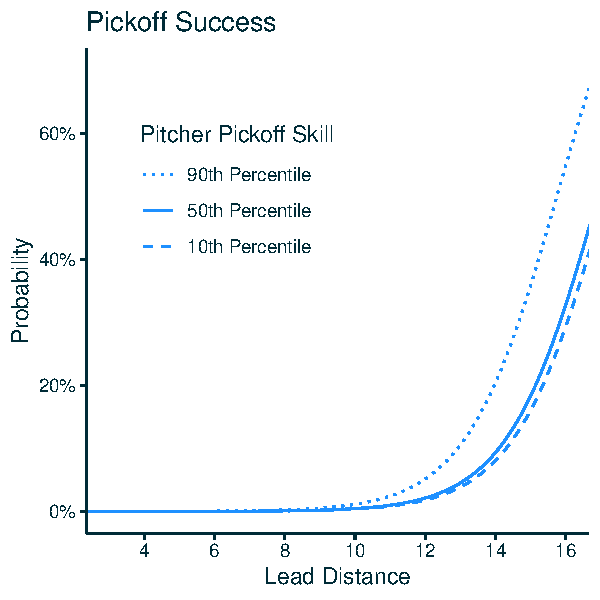
\includegraphics[width = 0.4\textwidth]{prob_po_success_light.pdf}
        \caption{
          \it Pickoff attempt probability (left) and success probability (right) modeled as functions of lead distance. The left figure corresponds to the model detailed from Section \ref{sec:prob-po-attempt}, assuming zero balls, zero strikes, zero outs, and a median pitcher random effect. The right figure corresponds to the model from Section \ref{sec:prob-po-success}, which includes only an intercept, a fixed effect for lead distance and a random effect for pitcher identity.
        }
        \label{fig:prob-pickoff}
      \end{figure}

      Figure \ref{fig:prob-sb-success} shows stolen base success probability modeled as a function of lead distance, split by season and by runner skill. We observe that, conditioned on lead distance, even 10$^\text{th}$-percentile runners in 2023 had higher success probabilities than the median runner in 2022, which is likely attributable to rule changes making it easier to steal bases in 2023. Within the range covering most lead distances, the difference between the 90$^\text{th}$-percentile runner and the median runner is just under 5 percentage points of success probability, similar to the difference between the median runner and the 10$^\text{th}$-percentile runner. Base-out state and battery (i.e. pitcher and catcher) skill also influence stolen base success probability although they are not shown in this visualization.
      
      \begin{figure}
        \centering
        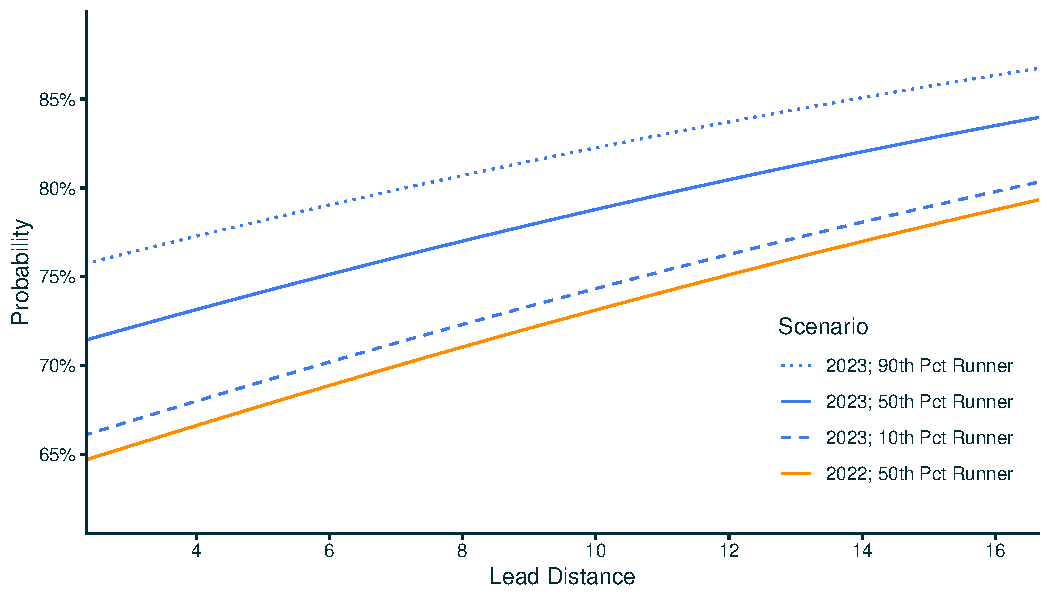
\includegraphics[width = 0.7\textwidth]{prob_sb_success_light.pdf}
        \caption{
          \it Stolen base success probability modeled as function of lead distance, split by season and runner effect (combining the fixed effect of runner sprint speed and the random effect of runner identity). This figure shows the probability estimated by the model detailed in Section \ref{sec:prob-sb-success}, assuming zero balls, zero strikes, zero outs, and a median value for the combined effect of pitcher identity (random effect), catcher arm strength (fixed effect), and catcher identity (random effect).
        }
        \label{fig:prob-sb-success}
      \end{figure}

      A novel \revision{applied result} of these runner outcome probability models \revision{stems from} the combination of fixed effects for measurable player characteristics (catcher arm strength and runner sprint speed) and random effects for player identities. This feature allows us to answer questions such as: How important are these measurable characteristics for player performance outcomes? And to what extent do players over- or under-perform what is expected from their measurable characteristics? The combination of the fixed effect and the random effect gives us an estimate (which we call the combined effect) of each player's skill, regularized toward what is expected from their measurable characteristics.

      For the stolen base success probability model, Figure \ref{fig:random-effect} shows the relationship between the combined player effect and the corresponding measurable characteristic, for both catchers and runners. We observe that arm strength explains 65\% of the variance in the catcher combined effect and that sprint speed explains 86\% of the variance in the runner combined effect. In other words, sprint speed tells us more about runner skill than arm strength tells us about catcher skill, with regard to stolen base outcomes. Beyond arm strength, the catcher can reduce stolen base success by releasing the ball more quickly or by throwing it more accurately to the target base. Beyond sprint speed, the runner can increase stolen base success by starting to run earlier (i.e., getting a better jump) or by accelerating more quickly to their top speed.
      
      \begin{figure}
        \centering
        
\includegraphics[width = 0.4\textwidth]{effect_catcher_light.pdf}
        
\includegraphics[width = 0.4\textwidth]{effect_runner_light.pdf}
        \caption{
          \it
          (Left) The relationship between arm strength and catcher combined effect on stolen base success probability (relative to average, on the log-odds scale). The combined effect is the sum of the fixed effect due to arm strength and the catcher random effect.
          (Right) The relationship between sprint speed and runner combined effect on stolen base success probability (relative to average, on the log-odds scale). The combined effect is the sum of the fixed effect due to sprint speed and the runner random effect.
        }
        \label{fig:random-effect}
      \end{figure}

    \subsection{Two-player sequential game}
    \label{sec:results-two-player}
    
      Using the transition probabilities estimated on the empirical data, we implemented the value iteration algorithm from Section \ref{sec:sg-model}, discretizing the runner's lead distance action space to the nearest tenth of a foot. Table \ref{tab:lead-by-count-two-player} reports how the optimal runner policy varies by count and disengagements, and Table \ref{tab:lead-by-outs-two-player} reports how the optimal runner policy varies by outs and disengagements. This runner policy maximizes runs scored while taking into account the rational behavior of both players, as defined by (\ref{eqn:sg_val}). For this runner policy, the pitcher is indifferent to attempting a pickoff or not.
      
      \begin{table}
        \resizebox{\textwidth}{!}{
          \inputtable{lead_by_count_two_player.tex}
        }
        \caption{
          \it The optimal lead distance (in feet) by count and prior disengagements under the two-player sequential game, assuming an average runner on first base facing an average battery (pitcher and catcher) with no outs and third base empty.
        }
        \label{tab:lead-by-count-two-player}
      \end{table}

      The most striking observation is that the optimal lead distance is significantly longer with two prior disengagements (14.9--15.8 feet) than in other states. These recommended lead distances are near the edge of observed lead distances in the dataset but not outside of the observed range. Overall, the optimal runner policy is more aggressive than observed behavior. Recall from Section \ref{sec:results-multilevel-model} that the average lead distance after zero, one, and two prior disengagements was 9.6 feet, 10.3 feet, and 11.0 feet, respectively.

      \begin{table}
        \small
        \centering       
        \inputtable{lead_by_outs_two_player.tex}
        \caption{
          \it The optimal lead distance (in feet) by outs and prior disengagements under the two-player sequential game, assuming an average runner on first base facing an average battery (pitcher and catcher) with an 0-0 count and third base empty.
        }
        \label{tab:lead-by-outs-two-player}
      \end{table}

      We observe that the lead distance generally, although not strictly, shortens as the count deepens (i.e., as the numbers of balls and strikes increase). This makes intuitive sense because the plate appearance is closer to ending, which relieves the pressure on the pitcher to avoid attempting a pickoff. The lead distance generally, although not strictly, increases as the number of outs increases. This makes intuitive sense because the runner is less likely to score without more aggressive action. In other words, the riskier lead distance is more palatable because the runner has a lower baseline probability of scoring from first base with two outs. The non-monotonicity of the optimal lead distance policy may be a consequence of estimating transition probabilities using empirical data.

      Under the game-theoretic equilibrium, pitchers would be more aggressive with attempting pickoffs when runners take long leads. Based on observed lead distances in 2023, we estimate that a pickoff attempt would be the optimal action in 11.4\% of opportunities with only first base occupied. When a pickoff attempt would have been recommended, pitchers attempted pickoffs 10.4\% of the time---100\% would be optimal. When a pickoff attempt would not have been recommended, pitchers attempted pickoffs 4.9\% of the time---0\% would be optimal. Overall, pitchers attempted pickoffs on 5.6\% of opportunities, less than the recommended 11.4\%.
      

      Despite the fact that pitchers would attempt more pickoffs under the game-theoretic equilibrium, Tables \ref{tab:lead-by-count-two-player} and \ref{tab:lead-by-outs-two-player} recommend longer leads for runners, particularly with two prior disengagements. The optimal strategy for the runner is maximin because they choose the lead distance which maximizes the minimum run expectancy across the pitcher's two options (pickoff or pitch). The pitcher will never attempt a pickoff when it is suboptimal to do so. The optimal behavior for the runner is to force their hand (or rather, to make the pitcher indifferent to their two choices).


    \subsection{One-player MDP}
    \label{sec:results-one-player}

      \revision{The results in Tables \ref{tab:lead-by-count-two-player} and \ref{tab:lead-by-outs-two-player} provide guidance to runners for choosing lead distances that are unexploitable from a game theory perspective. However,} pitchers may be unlikely to adapt their strategy to the optimal policy in the short term. Runner actions are already observable by the defense, and current pitcher behavior seems more conservative than optimal, as noted in Section \ref{sec:results-two-player}. After all, the pitcher has the additional cognitive burden of contending with the batter. In light of this, \revision{runners may achieve better results by choosing a policy to exploit observed pitcher behavior.}

      \revision{We consider replacing the pitcher's agency in the two-player sequential game with the probability model described in Section \ref{sec:prob-po-attempt}. The pickoff decision becomes a stochastic response to the runner's lead distance, resulting in a one-player MDP. As with the two-player game, we implement value iteration to find the optimal runner policy given observed pitcher behavior.} Table \ref{tab:lead-by-count-one-player} reports how the optimal policy varies by count and prior disengagements, and Table \ref{tab:lead-by-outs-one-player} reports how the optimal policy varies by outs and prior disengagements.

      \begin{table}
        \resizebox{\textwidth}{!}{
          \inputtable{lead_by_count_one_player.tex}
        }
        \caption{
          \it The optimal lead distance (in feet) by count and prior disengagements under the \revision{one}-player MDP, assuming an average runner on first base facing an average battery (pitcher and catcher) with no outs and third base empty.
        }
        \label{tab:lead-by-count-one-player}
      \end{table}

      For the most part, the trends in the optimal lead distance policy in the one-player MDP are similar to that of the two-player game. One exception is that optimal lead distance increases with the number of balls in the count because pitchers are less likely to attempt pickoffs (Table \ref{tab:model-summary}). The relationship between prior disengagements and optimal lead distance is also different. We observe that increasing prior disengagements from zero to one generally increases the optimal lead distance by approximately 1.5 feet. Increasing prior disengagements from one to two generally increases the optimal lead distance by approximately 2.5 feet.
      
      \begin{table}
        \small
        \centering
        \inputtable{lead_by_outs_one_player.tex}
        \caption{
          \it The optimal lead distance (in feet) by outs and prior disengagements under the \revision{one}-player MDP, assuming an average runner on first base facing an average battery (pitcher and catcher) with an 0-0 count and third base empty.
        }
        \label{tab:lead-by-outs-one-player}
      \end{table}
  
      Table \ref{tab:lead-by-players} shows the \revision{optimal runner policy by number of disengagements for different combinations of battery skill and runner skill.} Against batteries more skilled at controlling the run game, the optimal lead distance is shorter. For more skilled runners, the optimal lead distance is longer. \revision{However, the relationship between disengagements and recommenced lead distance is similar for different combinations of player skill. The first disengagement increases recommended lead distance by 0.9--1.7 feet, and the second disengagement results in an increase of 1.8--2.7 feet.}
    
      \begin{table}
        \small
        \centering
        \inputtable{lead_by_players.tex}
        \caption{
          \it Optimal lead distance (in feet) by battery/runner skill and prior disengagements, for an 0-0 count with no outs and third base empty. For example, the hypothetical 90$^\text{th}$-percentile battery represents the 90$^\text{th}$ percentile at attempting pickoffs, successfully executing pickoffs, suppressing stolen base attempts, and catching would-be base stealers.
        }
        \label{tab:lead-by-players}
      \end{table}

  \section{Discussion and \revision{actionable} insights}
  \label{sec:discussion}

    \revision{For coaches seeking a strategy for the lead distance problem to implement today, we recommend the optimal policy from the one-player MDP rather than the two-player game.} Pitchers are unlikely to immediately adapt their behavior to the optimal policy, and runners can exploit this. Because the pickoff attempt action is observable, runners can adjust their lead distance policy if they observe pitchers making \revision{different} pickoff decisions \revision{over time}.

    \revision{A simple approximation to the optimal policy} is the \textit{Two-Foot Rule}: Extend your lead by two feet after each pickoff attempt. \revision{Because runners already have significant cognitive burden in professional baseball games, it is essential to boil down our results into a memorable} and easily communicated rule of thumb. \revision{The Two-Foot Rule does not require consulting a chart to know what to do. It is a real-life actionable insight the would increase runner lead distances and increase run scoring.}

    Given observed lead distance behavior, offenses scored 0.516 runs per inning in 2023. In other words, if we model the inning as a Markov reward process using empirical transition probabilities between states, the value of the start-of-inning state is 0.516 runs. Under the two-player game, the value of the start-of-inning state is 0.520 runs, which corresponds to approximately 6 more runs over a full season of 162 games of nine innings each. Therefore, offenses stand to benefit more in the transition from observed behavior to a game-theoretic equilibrium. Under the one-player MDP, the value of the start-of-inning state is 0.524 runs, which corresponds to approximately 12 more runs over a full season, relative to observed behavior. Naturally, scoring expectation is higher in the one-player MDP because the runner exploits the sub-optimal strategy of the pitcher. To add 12 expected runs in free agency would cost roughly \$12 million \citep{clemens_what_2021}, which speaks to a significant (but not outlandish) impact. This value may have increased since the last study we found to have estimated it.

    In comparing the optimal lead distance policy under the two-player game (Table \ref{tab:lead-by-count-two-player}) and the \revision{one}-player MDP (Table \ref{tab:lead-by-count-one-player}), we observe substantial differences between them. For most states, the former lead distance is longer than the latter. The optimal policy for the runner under the two-player game is to extend their lead until the pitcher is indifferent between attempting a pickoff or not. By contrast, the one-player optimal policy corresponds to a pickoff attempt probability below 10\%. Because the pitcher sometimes attempts low-success pickoffs, the runner does not need to extend their lead further.

    In the two-player game we recommend long leads (beyond 15 feet) after two prior disengagements. These distances are near the edge of the range of leads we observe but not outside the range. To develop intuition for this policy, consider the optimal lead distance of 15.1 feet in a 3-2 count after two prior disengagements (Table \ref{tab:lead-by-count-two-player}). If an average pitcher attempts a pickoff in this scenario, we estimate a 20.5\% probability that the runner is out. Otherwise, the runner advances to second base. By contrast, if the pitcher throws a pitch and if the runner attempts a stolen base (14.0\% probability), we estimate an 82.8\% probability that the stolen base is successful. In other words, the pitcher is indifferent to throwing a pitch or attempting a pickoff because the probability of an unsuccessful pickoff attempt is similar to the probability of a successful stolen base (conditioned on a steal attempt), and the outcome is the same either way.

    Because a third failed pickoff attempt results directly in free baserunner advancement, the pitcher is strongly disincentivized from attempting a pickoff after two prior disengagements. In the two-player game, this is reflected in a drastic increase in the optimal lead distance after the second disengagement (3--5 feet, Table \ref{tab:lead-by-count-two-player}). In the one-player MDP, we observe a more steady increase in optimal lead distance as a function of prior disengagements because observed pitcher pickoff attempt behavior steadily decreases as a function of prior disengagements (see Figure \ref{fig:prob-pickoff}).
    
  \section{Conclusion}

    Under the new pickoff rules, baseball players and coaches understand intuitively that runners want to increase their lead distance after each successive disengagement by the pitcher---but by how much? In this paper, we formalize the cat-and-mouse game between pitcher and runner as a two-player sequential game and estimate the optimal lead distance policy for a runner on first base with other bases empty, given the number of outs, the ball-strike count, and the number of prior disengagements by the pitcher. We model the probabilities of runner outcomes (pickoff attempt/success, stolen base attempt/success) as functions of lead distance, context, and player skill. This allows us to estimate the optimal lead distance policy for any combination of pitcher skill and runner skill.

    We consider a two-player sequential game in which the runner first decides their lead distance and then the pitcher (upon observing the runner's lead distance) then decides whether to attempt a pickoff or throw a pitch. We show that the game-theoretic optimal policy for the runner is a maximin strategy (with respect to rest-of-inning run expectancy) so that the pitcher is indifferent to attempting a pickoff or throwing a pitch. We estimate model parameters using empirical data from the 2023 MLB season and find that under the game-theoretic equilibrium, runners would be more aggressive with their lead distances than the current behavior we observe. While baseball analytics sometimes garners negative attention for diminishing the aesthetic appeal of the game \citep{sheinin_analytics_2025}, this is an example for which the analytically recommended strategy could be more aesthetically pleasing. In other sports, stochastic and dynamic models have shown that decision-makers have been traditionally too conservative \citep{romer_firms_2006, beaudoin_strategies_2010, yam_what_2019}, but this is a new result for leadoff and pickoff decisions baseball.

    We go a step further and consider the opportunity for runners to exploit the observed suboptimal behavior by pitchers. We consider a one-player MDP in which the pitcher's agency in the pickoff decision is replaced by a stochastic process, modeled on empirical data as a function of the runner's lead distance.  This framework leads to the most actionable recommendation for runners under the current conditions of pitcher behavior. We estimate that the average team could expect to increase their expected offensive output by approximately 12 runs over a full season by implementing the optimal lead distance policy. Based on these results, we propose the Two-Foot Rule: Extend your lead by two feet after each pickoff attempt. This easily implemented recommendation is a good approximation to the optimal lead distance policy across a wide array of contexts (outs and ball-strike count) and pitcher/runner skills.

    Our results come with some simplifying assumptions that are necessary limitations given the data available. We assume that observed lead distance fully describes the runner's behavior and that they cannot disguise their aggressiveness by leaning in one direction. In reality, the runner may achieve a greater (or lesser) effective lead distance than we observe by leaning toward second base (or first base). We also assume that lead distance only impacts pickoff and stolen base outcomes, not the outcomes of batted balls. For example, we assume that a greater lead distance does not improve the runner's probability of advancing from first base to third base on a single. Baseball domain knowledge suggests this is a reasonable assumption because while a pitch is being thrown, the runner moves to a secondary lead distance which is more important than primary lead distance for determining advancement outcomes. Finally, we assume that, other than pickoff attempts, no other disengagements occur. In reality, the pitcher may derive value from stepping off the pitching rubber if they are short of breath or need to resolve a miscommunication with the catcher. These extensions are opportunities for future work. Another future direction is to model an entire roster, which is a nonstationary two-player sequential game and introduces enormous technical challenges.

    In addition to the lead distance data used in the current work, which is based on the runner's center of mass, MLB has begun collecting 18-point pose tracking data on runners and fielders at 50 frames per second \citep{jedlovec_introducing_2020}. If these data were publicly available, they would enable more granular modeling of the cat-and-mouse game between pitcher and runner. For example, with information about the runner's leaning posture and reaction time, future work might show that a mixed strategy for the pitcher's pickoff decision achieves the best result by forcing a neutral posture for the runner and delaying the runner's reaction. As highlighted in Section \ref{sec:prob-sb-attempt}, another opportunity for future work is improved modeling of the runner's decision to attempt a stolen base, which we assumed to be stochastic and independent of lead distance.

  \section*{Acknowledgments}

    Major League Baseball trademarks and copyrights are used with permission of MLB Advanced Media, L.P. All rights reserved. The authors thank Mallesh Pai of Rice University for constructive discussions during conceptualization of the problem and early implementation of the solution.

  \section*{Code and data availability}

    Code related to this paper is available at \url{https://github.com/jfhahn2/pickoff-game-theory}. Lead distance data are not publicly available and were obtained from MLB Advanced Media. All other data are publicly available and may be downloaded using the R package sabRmetrics \citep{powers_sabrmetrics_2025}.


%%%%%%%%%%%%%%%%%%%%%%%%%%%%%%%%%%%%%%%%%%%%%%
%% Appendix---Please move all appendices to %%
%% a Supplementary file.                    %%
%%%%%%%%%%%%%%%%%%%%%%%%%%%%%%%%%%%%%%%%%%%%%%
%% Support information, if any,             %%
%% should be provided in the                %%
%% Acknowledgements section.                %%
%%%%%%%%%%%%%%%%%%%%%%%%%%%%%%%%%%%%%%%%%%%%%%
%\begin{acks}[Acknowledgments]
% The authors would like to thank ...
%\end{acks}
%%%%%%%%%%%%%%%%%%%%%%%%%%%%%%%%%%%%%%%%%%%%%%
%% Funding information, if any,             %%
%% should be provided in the                %%
%% funding section.                         %%
%%%%%%%%%%%%%%%%%%%%%%%%%%%%%%%%%%%%%%%%%%%%%%
%\begin{funding}
% The first author was supported by ...
%
% The second author was supported in part by ...
%\end{funding}

%%%%%%%%%%%%%%%%%%%%%%%%%%%%%%%%%%%%%%%%%%%%%%
%% Supplementary Material, including data   %%
%% sets and code, should be provided in     %%
%% {supplement} environment with title      %%
%% and short description. It cannot be      %%
%% available exclusively as external link.  %%
%% All Supplementary Material must be       %%
%% available to the reader on Project       %%
%% Euclid with the published article.       %%
%%%%%%%%%%%%%%%%%%%%%%%%%%%%%%%%%%%%%%%%%%%%%%
%\begin{supplement}
%\stitle{???}
%\sdescription{???.}
%\end{supplement}

%%%%%%%%%%%%%%%%%%%%%%%%%%%%%%%%%%%%%%%%%%%%%%%%%%%%%%%%%%%%%
%%                  The Bibliography                       %%
%%                                                         %%
%%  imsart-nameyear.bst  will be used to                   %%
%%  create a .BBL file for submission.                     %%
%%                                                         %%
%%  Note that the displayed Bibliography will not          %%
%%  necessarily be rendered by Latex exactly as specified  %%
%%  in the online Instructions for Authors.                %%
%%                                                         %%
%%  MR numbers will be added by VTeX.                      %%
%%                                                         %%
%%  Use \cite{...} to cite references in text.             %%
%%                                                         %%
%%%%%%%%%%%%%%%%%%%%%%%%%%%%%%%%%%%%%%%%%%%%%%%%%%%%%%%%%%%%%

%% if your bibliography is in bibtex format, uncomment commands:
\bibliographystyle{imsart-nameyear} % Style BST file
\bibliography{articles/bibliography}       % Bibliography file (usually '*.bib')

%% or include bibliography directly:
% \begin{thebibliography}{}
% \bibitem[\protect\citeauthoryear{???}{???}]{b1}
% \end{thebibliography}

\end{document}
